%%
%% Start Definitions (each of these we can reuse)
%%

\begin{SaveDefinition}[key=FundamentalSubspaces, title={Fundamental Subspaces}]
	\index{Matrix!fundmamental subspaces of}\index[definitions]{Matrix!fundamental subspaces of}
	Associated with any matrix $M$ are three fundamental subspaces: the
	\emph{row space}\index{Matrix!row space}\index[definitions]{Matrix!row space} of $M$, denoted $\Row(M)$\index[symbols]{$\Row(M)$}, is the span of the rows of
	$M$; the
	\emph{column space}\index{Matrix!column space}\index[definitions]{Matrix!column space} of $M$, denoted $\Col(M)$\index[symbols]{$\Col(M)$}, is the span of the
	columns of $M$; and the
	\emph{null space}\index{Matrix!null space}\index[definitions]{Matrix!null space} of $M$, denoted $\Null(M)$\index[symbols]{$\Null(M)$}, is the set of solutions to
	$M\vec x=\vec 0$.
\end{SaveDefinition}

\begin{SaveDefinition}[key=RankofaLinearTransformation, title={Rank of a Linear Transformation}]
	For a linear transformation $T:\R^n\to \R^m$, the
	\emph{rank}\index[definitions]{Linear transformation!rank}\index{Linear transformation!rank} of $T$, denoted $\Rank(T)$\index[symbols]{$\Rank(T)$}, is the dimension of the range of
	$T$.
\end{SaveDefinition}

\begin{SaveDefinition}[key=RankofaMatrix, title={Rank of a Matrix}]
	Let $M$ be a matrix.
	The \emph{rank}\index[definitions]{Matrix!rank}\index{Matrix!rank} of $M$, denoted $\Rank(M)$\index[symbols]{$\Rank(M)$}, is the rank of
	the linear transformation induced by $M$.
\end{SaveDefinition}

\begin{SaveDefinition}[key=NullityofaMatrix, title={Nullity of a Matrix}]
	Let $M$ be a matrix.
	The \emph{nullity}\index[definitions]{Matrix!nullity}\index{Matrix!nullity} of $M$, denoted $\Nullity(M)$\index[symbols]{$\Nullity(M)$}, is the nullity of
	the linear transformation induced by $M$.
\end{SaveDefinition}

\begin{SaveDefinition}[key=Rank, title={Rank}]
	For a linear transformation $T:\R^n\to \R^m$, the
	\emph{rank} of $T$, denoted $\Rank(T)$, is the dimension of the range of
	$T$.\index[definitions]{Linear transformation!rank}\index{Linear transformation!rank}

	For an $m\times n$ matrix $M$, the
	\emph{rank} of $M$, denoted $\Rank(M)$, is the dimension of the 
	column space of $M$.\index[definitions]{Matrix!nullity}\index{Matrix!nullity}
\end{SaveDefinition}

\begin{SaveDefinition}[key=Nullity, title={Nullity}]
	For a linear transformation $T:\R^n\to \R^m$, the
	\emph{nullity} of $T$, denoted $\Nullity(T)$, is the dimension of the null space of
	$T$.\index[definitions]{Linear transformation!nullity}\index{Linear transformation!nullity}
\end{SaveDefinition}

\begin{SaveDefinition}[key=ChangeofBasisMatrix, title={Change of Basis Matrix}]
	Let $\mathcal A$ and $\mathcal B$ be bases for $\R^n$. The matrix $M$ is called
	a \emph{change of basis} matrix\index[definition]{Change of basis matrix}\index{Change of basis matrix} (which converts from $\mathcal A$ to $\mathcal B$) if
	for all $\vec x\in \R^n$
	\[
		M[\vec x]_{\mathcal A}=[\vec x]_{\mathcal B}.
	\]
	 Notationally, $\BasisChange{\mathcal A}{\mathcal B}$\index[symbols]{$\protect\BasisChange{\mathcal A}{\mathcal B}$}
	stands for the change of basis matrix converting from $\mathcal A$ to $\mathcal B$,
	and we may write $M=\BasisChange{\mathcal A}{\mathcal B}$.
\end{SaveDefinition}

\begin{SaveDefinition}[key=LinearTransformationinaBasis, title={Linear Transformation in a Basis}]
	Let $\mathcal T:\R^n\to\R^n$ be a linear transformation and let $\mathcal B$ be a
	basis for $\R^n$. The \emph{matrix for $\mathcal T$ with respect to $\mathcal B$}, notated
	$[\mathcal T]_{\mathcal B}$,
	is the $n\times n$ matrix satisfying
	\[
		[\mathcal T\vec x]_{\mathcal B} = [\mathcal T]_{\mathcal B}[\vec x]_{\mathcal B}.
	\]
	In this case, we say the matrix $[\mathcal T]_{\mathcal B}$\index[symbols]{$[\mathcal T]_{\mathcal B}$} is the representation
	of $\mathcal T$ in the $\mathcal B$ basis.
	\index{Matrix!of a linear transformation}\index[definitions]{Matrix!of a linear transformation}\index{Linear transformation!representation in a basis}\index[definitions]{Linear transformation!representation in a basis}
\end{SaveDefinition}

\begin{SaveDefinition}[key=SimilarMatrices, title={Similar Matrices}]
	The matrices $A$ and $B$ are called
	\emph{similar matrices}\index[definitions]{Matrix!similar matrices},
	denoted $A\sim B$\index[symbols]{$\sim$}, if $A$ and $B$ represent the
	same linear transformation but in possibly different bases. Equivalently,
	$A\sim B$ if there is an invertible matrix $X$ so that
	\[
		A=XBX^{-1}.
	\]

\end{SaveDefinition}


\begin{SaveDefinition}[key=Determinant, title={Determinant}]
	The
	\emph{determinant}\index{Determinant}\index[definitions]{Determinant} of a linear transformation $\mathcal T:\R^{n}\to \R^{n}$, denoted $\det(\mathcal T)$\index[symbols]{$\det(\mathcal T)$} or $\Abs{\mathcal T}$\index[symbols]{$\Abs{\mathcal T}$}, is
	the oriented volume of the image of the unit $n$-cube. The determinant of
	a square matrix is the determinant of its induced transformation.
\end{SaveDefinition}

\begin{SaveDefinition}[key=OrientationPreservingLinearTransformation, title={Orientation Preserving Linear Transformation}]
	Let $\mathcal T:\R^n\to\R^n$ be a linear transformation. We say $\mathcal T$
	is \emph{orientation preserving}\index[definitions]{Linear transformation!orientation preserving}\index{Linear transformation!orientation preserving} if the ordered basis $\Set{\mathcal T(\vec e_1),\ldots, \mathcal T(\vec e_n)}$
	is positively oriented  and we say $\mathcal T$
	is \emph{orientation reversing}\index[definitions]{Linear transformation!orientation reversing}\index{Linear transformation!orientation reversing} if the ordered basis $\Set{\mathcal T(\vec e_1),\ldots, \mathcal T(\vec e_n)}$
	is negatively oriented. If $\Set{\mathcal T(\vec e_1),\ldots, \mathcal T(\vec e_n)}$
	is not a basis for $\R^n$, then $\mathcal T$ is neither orientation preserving nor orientation reversing.
\end{SaveDefinition}

\begin{SaveDefinition}[key=Eigenvector, title={Eigenvector}]
	Let $X$ be a linear transformation or a matrix. An
	\emph{eigenvector}\index[definitions]{Eigenvector}\index{Eigenvector} for $X$ is a non-zero vector that doesn't change
	directions when $X$ is applied. That is, $\vec v\neq \vec 0$ is an
	eigenvector for $X$ if
	\[
		X\vec v=\lambda \vec v
	\]
	 for some scalar $\lambda$. We call $\lambda$ the
	\emph{eigenvalue}\index[definitions]{Eigenvalue}\index{Eigenvalue} of $X$ corresponding to the eigenvector $\vec v$.
\end{SaveDefinition}

\begin{SaveDefinition}[
	key=CharacteristicPolynomial,
	title={Characteristic Polynomial}]

	For a matrix $A$, the
	\emph{characteristic polynomial}\index{Characteristic polynomial}\index[definition]{Characteristic Polynomial} of $A$ is
	\[
		\chr(A)=\det(A-\lambda I).
	\]\index[symbols]{$\chr(A)$}

\end{SaveDefinition}

\begin{SaveDefinition}[key=Diagonalizable, title={Diagonalizable}]
	A matrix is
	\emph{diagonalizable}\index{Matrix!diagonalizable}\index[definitions]{Matrix!diagonalizible} if it is similar to a diagonal matrix.
\end{SaveDefinition}

\begin{SaveDefinition}[key=Eigenspace, title={Eigenspace}]
	Let $A$ be an $n\times n$ matrix with eigenvalues
	$\lambda_{1},\ldots,\lambda_{m}$. The
	\emph{eigenspace}\index[definitions]{Eigenspace}\index{Eigenspace} of $A$ corresponding to the eigenvalue $\lambda_{i}$
	is the null space of $A-\lambda_{i} I$. That is, it is the space spanned
	by all eigenvectors that have the eigenvalue $\lambda_{i}$.

	The
	\emph{geometric multiplicity}\index[definitions]{Eigenvalue!geometric multiplicity}\index{Eigenvalue!geometric multiplicity} of an eigenvalue $\lambda_{i}$ is the
	dimension of the corresponding eigenspace. The
	\emph{algebraic multiplicity}\index[definitions]{Eigenvalue!algebraic multiplicity}\index{Eigenvalue!algebraic multiplicity} of $\lambda_{i}$ is the number of times
	$\lambda_{i}$ occurs as a root of the characteristic polynomial of $A$ (i.e.,
	the number of times $x-\lambda_{i}$ occurs as a factor).
\end{SaveDefinition}


\begin{SaveDefinition}[key=Diagonal, title={Diagonal}]
	The \emph{diagonal}\index[definitions]{Matrix!diagonal of} of an $m\times n$ matrix $A=[a_{ij}]$ consists of
	the entries $a_{ij}$ satisfying $i=j$.
\end{SaveDefinition}
\begin{SaveDefinition}[key=SquareMatrix, title={Square Matrix}]
	A matrix is called \emph{square}\index[definitions]{Matrix!square} if it has the same
	number of rows as columns.
\end{SaveDefinition}
\begin{SaveDefinition}[key=DiagonalMatrix, title={Diagonal Matrix}]
	A square matrix is called \emph{diagonal}\index[definitions]{Matrix!diagonal} the only non-zero
	entries in the matrix appear on the diagonal.
\end{SaveDefinition}
\begin{SaveDefinition}[key=TriangleOf, title={Upper \& Lower Triangle}]
	Let $A=[a_{ij}]$ be an $m\times n$ matrix. The \emph{upper triangle}\index[definitions]{Matrix!upper triangle of}
	of $A$ consists the entries $a_{ij}$
	satisfying $j\geq i$. The \emph{lower triangle}\index[definitions]{Matrix!lower triangle of}
	of $A$ consists of the entries $a_{ij}$ satisfying $j\leq i$.
\end{SaveDefinition}
\begin{SaveDefinition}[key=TriangularMatrix, title={Triangular Matrices}]
	A matrix is called \emph{upper triangular}\index[definitions]{Matrix!upper triangular} if all non-zero entries lie in the upper triangle of the matrix and
	a matrix is called \emph{lower triangular}\index[definitions]{Matrix!lower triangular} if all non-zero entries lie in the lower triangle. A matrix is
	called \emph{triangular}\index[definitions]{Matrix!triangular} if it is either upper or lower triangular.
\end{SaveDefinition}
\begin{SaveDefinition}[key=SymmetricMatrix, title={Symmetric Matrix}]
	The square matrix $A=[a_{ij}]$ is called \emph{symmetric}\index[definitions]{Matrix!symmetric} if its
	entries satisfy $a_{ij}=a_{ji}$.

	Alternatively, if the entries of $A$ satisfy $a_{ij}=-a_{ji}$, then $A$
	is called \emph{skew-symmetric} or \emph{anti-symmetric}\index[definitions]{Matrix!skew-symmetric}.
\end{SaveDefinition}
\begin{SaveDefinition}[key=ZeroMatrix, title={Zero Matrix}]
	A matrix is called a \emph{zero matrix}\index[definitions]{Matrix!zero matrix} if all its entries are zero.
\end{SaveDefinition}
\begin{SaveDefinition}[key=PhasePortrait, title={Phase Portrait}]
		A \emph{phase portrait}\index[definitions]{phase!portrait} or \emph{phase diagram}\index[definitions]{phase!diagram} is the plot of a vector field in phase space
		where each vector rooted at $(x,y)$ is tangent to a solution curve passing through $(x,y)$
		and its length is given by the speed of a solution passing through $(x,y)$.
\end{SaveDefinition}



%%%%%%%%%%%%%%%%%%%%%%%%%%%%% ODEs %%%%%%%%%%%%%%%%%%%%%%%%%%%%%


\begin{SaveDefinition}[key=ClassificationOfEquilibria, title={Classification of Equilibria}]
		An equilibrium solution $f$ is called
		\begin{itemize}
			\item \emph{attracting}\index[definitions]{equilibrium!attracting} if locally solutions converge to $f$
			\item \emph{repelling}\index[definitions]{equilibrium!repelling} if there is a fixed distance so that locally, solutions tend away from $f$ by that fixed distance
			\item \emph{stable}\index[definitions]{equilibrium!stable} if there is a fixed distance so that locally, solutions stay within that fixed distance of $f$
			\item \emph{unstable}\index[definitions]{equilibrium!unstable} if $f$ is not stable
		\end{itemize}
\end{SaveDefinition}

\begin{SaveDefinition}[key=ClassificationOfEquilibriaFormal, title={Classification of Equilibria (Formal)}]
		An equilibrium solution $f$ is called
		\begin{itemize}
			\item \emph{attracting at time $t_0$}\index[definitions]{equilibrium!attracting} if 
			there exists $\varepsilon >0$ such that for all solutions $g$ satisfying $\abs{g(t_0)-f(t_0)} < \varepsilon$, we have $\lim_{t\to\infty} f(t)=\lim_{t\to\infty} g(t)$.

			\item \emph{repelling at time $t_0$}\index[definitions]{equilibrium!repelling} if there exists $\varepsilon>0$ and $\delta>0$ such that for all
			solutions $g$ that satisfy $0<\abs{g(t_0)-f(t_0)}<\varepsilon$ there exists $T\in \R$ so that for all $t>T$ we have
			$\abs{g(t)-f(t)}>\delta$

			\item \emph{stable at time $t_0$}\index[definitions]{equilibrium!stable} if for all $\varepsilon>0$ there exists a $\delta>0$ such that for all $g$ satisfying $\abs{g(t_0)-f(t_0)}<\delta$
			we have $\abs{g(t)-f(t)}<\varepsilon$ for all $t>t_0$.

			\item \emph{unstable at time $t_0$}\index[definitions]{equilibrium!unstable} if $f$ is not stable at time $t_0$
		\end{itemize}
		$f$ is called attracting/repelling/stable/unstable if it has the corresponding property for all $t$.
\end{SaveDefinition}


\begin{SaveDefinition}[key=ComponentGraphAndPhasePlane, title={Component Graph \& Phase Plane}]
	For a differential equation involving the functions $F_1$, $F_2$, \ldots, $F_n$, and the variable $t$,
	the \emph{component graphs}\index[definitions]{component graph} are the $n$ graphs of $(t, F_1(t))$, $(t, F_2(t))$, \ldots.
	
	The \emph{phase plane}\index[definitions]{phase!plane} or \emph{phase space}\index[definitions]{phase!space} associated with the differential equation
	is the $n$-dimensional space with axes corresponding to
	the values of $F_1$, $F_2$, \ldots, $F_n$.
\end{SaveDefinition}

\begin{SaveDefinition}[key=ClassificationOfEquilibria, title={Classification of Equilibria}]
		An equilibrium solution $f$ is called
		\begin{itemize}
			\item \emph{attracting}\index[definitions]{equilibrium!attracting} if locally solutions converge to $f$
			\item \emph{repelling}\index[definitions]{equilibrium!repelling} if there is a fixed distance so that locally, solutions tend away from $f$ by that fixed distance
			\item \emph{stable}\index[definitions]{equilibrium!stable} if there is a fixed distance so that locally, solutions stay within that fixed distance of $f$
			\item \emph{unstable}\index[definitions]{equilibrium!unstable} if $f$ is not stable
		\end{itemize}
\end{SaveDefinition}

%%%%%%%%%%%%%%%%%%%%%%%%%%%%% Math Modelling %%%%%%%%%%%%%%%%%%%%%%%%%%%%%

\begin{SaveDefinition}[key=FundamentalDimensions, title={Seven Fundamental Dimensions}]

There are seven fundamental dimensions: \\

\begin{tabular}{cccc}
Dimension & Symbol & \multicolumn{2}{c}{SI Unit}   \\ \hline
length & $L$ & metre & m \\
mass & $M$ & kilogram & kg \\
time & $T$ & second & s \\
electric current & $I$ & ampere & A \\
temperature & $\Theta$ & kelvin & K \\
amount & $N$ & mole & mol \\
light intensity & $J$ & candela & cd
\end{tabular} \\

\textit{Note: } Sometimes, we use charge $Q$ (SI Unit coulomb C) as a fundamental dimension instead of current.
\end{SaveDefinition}


\begin{SaveDefinition}[key=DimensionalMatrix, title={Dimensional Matrix}]
	The dimensional matrix $\mathcal{D}$ is a matrix where its $(i,j)$ entry gives the power of the $i^{\rm th}$ dimension of the $j^{\rm th}$ variable.
\end{SaveDefinition}

\begin{SaveDefinition}[key=BuckinghamPiThm, title={Buckingham Pi Theorem}]
	Any physical relation involving $N$ dimensional variables can be written in terms of a complete set of $N - r$ independent dimensionless variables, where $r$ is the rank of the dimensional matrix $\mathcal{D}$.
		
	The notational convention for the Buckingham Pi Theorem is that the ``pi's'', $\Pi_1,\ldots, \Pi_{N-r}$ represent dimensionless variables and a relation between them is given by $F(\Pi_1,\ldots,\Pi_{N-r}) = 0$.
\end{SaveDefinition}


\begin{SaveDefinition}[key=Sensitivity, title={Parameter Sensitivity}]

Parameter sensitivity is a measure of how a model's response is affected by its parameters.

We quantify the \textbf{sensitivity} for the model output $x$ and model parameter $p$ by
\[
S(x,p) = \frac{\partial x}{\partial p} \cdot \frac{p}{x},
\]
which is dimensionless.
\end{SaveDefinition}



\begin{SaveDefinition}[key=Newton1, title={Newton's Method}]

This is a method to approximate the solution of the equation
\[
f(x)=0.
\]

This is an iterative method, so we start with an initial approximation $x_0$.

For each successive approximation, take the linear approximation of $f$ at $x_i$ and take $x_{i+1}$ to be the point where the linear approximation is 0.
\end{SaveDefinition}


\begin{SaveDefinition}[key=Newton, title={Newton's Method}]

This is a method to approximate the solution of the equation
\[
f(x)=0,
\]
from an initial guess $x_0$.

For each successive approximation, take the linear approximation of $f$ at $x_i$ and take $x_{i+1}$ to be the point where the linear approximation is 0.

This means that 
\[
x_{n+1} = x_n - \frac{f(x_n)}{f'(x_n)}.
\]
\end{SaveDefinition}



\begin{SaveDefinition}[key=LagrangeMultipliers, title={Lagrange Multipliers}]

We want to minimize (or maximize) a function $f(x)$ with several constraints:
	\begin{align*}
		g_1(x) 	& = c_1 \\
				& \vdots \\
		g_k(x) 	& = c_k
	\end{align*}

\textbf{If} $x^\star \in \R^N$ is a local optimal of $f(x)$ which satisfies the above constraints, and $\nabla g_1(x^\star), \ldots, \nabla g_k(x^\star)$ are linearly independent, \textbf{then}
\[
\nabla f(x^\star) = \lambda_1 \nabla g_1(x^\star) + \cdots + \lambda_k \nabla g_k(x^\star),
\tag{LM}\label{LM}
\]
for some scalars $\lambda_1, \ldots, \lambda_k$.
\end{SaveDefinition}




\begin{SaveDefinition}[key=EulerLagrange, title={Euler-Lagrange Equation}]

The minimizer $x^\star(t)$ of the functional
\[ \min \int_{t_0}^{t_1} F \big(t, x(t), x'(t) \big) ~dt \]
with $x(t_0)=x_0$ and $x(t_1)=x_1$ satisfies the \textbf{Euler-Lagrange Equation}:
\[
\frac{\partial F}{\partial x} (t, x^\star, {x^\star}')
	= \frac{d}{dt} \frac{\partial F}{\partial x'} (t, x^\star, {x^\star}') .
\]

%Note: This is a necessary but not sufficient condition.
\end{SaveDefinition}




\begin{SaveDefinition}[key=EulerMethod, title={Euler Method}]
\begin{align*}
y_{n+1} & = y_n + h k_1\\	
k_1 & = f(t_n, y_n)
\end{align*}

\begin{center}
\begin{tikzpicture}
	\draw[latex-latex] (4,0) -- (0,0) -- (0,4);
    \draw[dashed] (1,0) node[below] {$t_n$} -- (1,4);
    \draw[dashed] (2,0) -- (2,4);
    \draw[dashed] (3,0) node[below] {$t_{n+1}$} -- (3,4);
    \draw[dashed] (0,2) node[left] {$y_n$} -- (4,2);
	\draw[fill=gray] (1,2) circle (0.1);
    \draw[blue!50!black, fill=blue!50!white] (3,3) circle (0.1);
    \draw[-latex, thick, blue!50!black] (1,2) -- node[above] {$k_1$} (3,3);
\end{tikzpicture}
\end{center}
\end{SaveDefinition}


\begin{SaveDefinition}[key=HeunMethod, title={Heun Method (Improved Euler)}]

\begin{align*}
y_{n+1} & = y_n + h \frac{k_1 + k_2}{2} \\	
k_1 & = f(t_n, y_n) \\
k_2 & = f(t_n+h, y_n + h k_1)
\end{align*}

\begin{center}
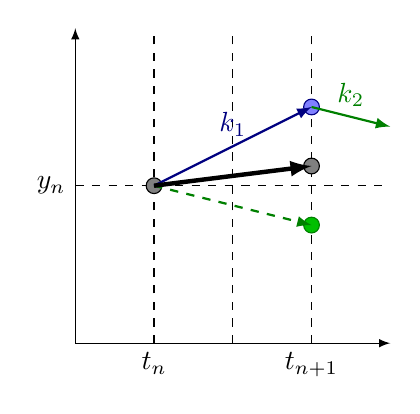
\begin{tikzpicture}
	\draw[latex-latex] (4,0) -- (0,0) -- (0,4);
    \draw[dashed] (1,0) node[below] {$t_n$} -- (1,4);
    \draw[dashed] (2,0) -- (2,4);
    \draw[dashed] (3,0) node[below] {$t_{n+1}$} -- (3,4);
    \draw[dashed] (0,2) node[left] {$y_n$} -- (4,2);
	\draw[fill=gray] (1,2) circle (0.1);
    \draw[blue!50!black, fill=blue!50!white] (3,3) circle (0.1);
    \draw[-latex, thick, blue!50!black] (1,2) -- node[above] {$k_1$} (3,3);
    \draw[-latex, thick, green!50!black] (3,3) -- node[above] {$k_2$} (4,2.75);
    \draw[green!50!black, fill=green!75!black] (3,1.5) circle (0.1);
    \draw[-latex,dashed, thick, green!50!black] (1,2) -- (3,1.5);    
    \draw[fill=gray] (3,{(3+1.5)/2}) circle (0.1);
    \draw[-latex, ultra thick] (1,2) -- (3,{(3+1.5)/2});
\end{tikzpicture}
\end{center}

\end{SaveDefinition}


\begin{SaveDefinition}[key=RK4Method, title={Runge-Kutta Method (4$^{\text{th}}$ order)}]

\begin{minipage}{.6\textwidth}
\begin{align*}
y_{n+1} & = y_n + h \frac{k_1 + 2k_2+2k_3 + k_4}{6} \\	
k_1 & = f(t_n, y_n) \\
k_2 & = f(t_n+\frac{h}{2}, y_n + \frac{h}{2} k_1) \\
k_3 & = f(t_n+\frac{h}{2}, y_n + \frac{h}{2} k_2) \\
k_4 & = f(t_n+h, y_n + h k_3)
\end{align*}
\end{minipage}
\hfil
\begin{minipage}{.3\textwidth}
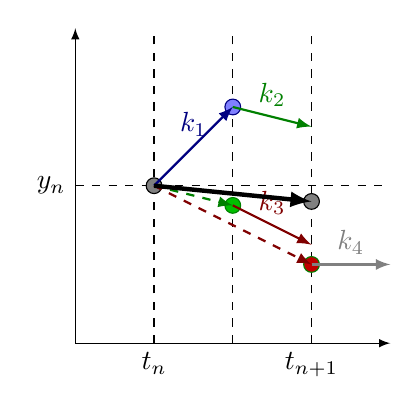
\begin{tikzpicture}
	\draw[latex-latex] (4,0) -- (0,0) -- (0,4);
    \draw[dashed] (1,0) node[below] {$t_n$} -- (1,4);
    \draw[dashed] (2,0) -- (2,4);
    \draw[dashed] (3,0) node[below] {$t_{n+1}$} -- (3,4);
    \draw[dashed] (0,2) node[left] {$y_n$} -- (4,2);
	\draw[fill=gray] (1,2) circle (0.1);
    \draw[blue!50!black, fill=blue!50!white] (2,3) circle (0.1);
    \draw[-latex, thick, blue!50!black] (1,2) -- node[above] {$k_1$} (2,3);
    \draw[-latex, thick, green!50!black] (2,3) -- node[above] {$k_2$} (3,2.75);
    \draw[green!50!black, fill=green!75!black] (2,1.75) circle (0.1);
    \draw[-latex,dashed, thick, green!50!black] (1,2) -- (2,1.75);    
    \draw[-latex, thick, red!50!black] (2,1.75) -- node[above] {$k_3$} (3,1.25);    
    \draw[green!50!black, fill=red!75!black] (3,1) circle (0.1);
    \draw[-latex,dashed, thick, red!50!black] (1,2) -- (3,1); 
    \draw[-latex, thick, gray] (3,1) -- node[above] {$k_4$} (4,1);
    \draw[fill=gray] (3,1.8) circle (0.1);
    \draw[-latex, ultra thick] (1,2) -- (3,1.8);
\end{tikzpicture}
\end{minipage}
\end{SaveDefinition}



\begin{SaveDefinition}[key=bifurcations, title={Bifurcations}]

A (local) \textbf{bifurcation} occurs when a parameter change causes the stability of an equilibrium to change.

We will study four typical types of bifurcations.

\begin{enumerate}
	\item \textbf{Saddle-node bifurcation}. Two equilibria collide and annihilate each other.
	\item \textbf{Transcritical bifurcation}. An equilibrium exists for all values of a parameter and is never destroyed. However, the equilibrium interchanges its stability with another equilibrium as the parameter changes.
	\item \textbf{Pitchfork bifurcation}. One equilibrium transitions to three equilibria as a parameter changes.
	\item \textbf{Hopf bifurcation}. A periodic orbit appears (or disappears) through a change in the stability of an equilibrium point -- this means that we transition from purely imaginary to complex eigenvalues.
\end{enumerate}


\end{SaveDefinition}




